\documentclass[11pt]{article}
 
\usepackage[utf8]{inputenc} % allow utf-8 input
\usepackage[T1]{fontenc}    % use 8-bit T1 fonts
\usepackage{hyperref}       % hyperlinks
\usepackage{url}            % simple URL typesetting
\usepackage{booktabs}       % professional-quality tables
\usepackage{amsfonts}       % blackboard math symbols
\usepackage{nicefrac}       % compact symbols for 1/2, etc.
\usepackage{microtype}      % micro typography
\usepackage{xcolor}         % colors
\usepackage{tikz}           % drawings
\usepackage{pgfplots}       % plots
\usepackage{xfrac}          % better fractions
\usepackage{subcaption}      % figure-in-figure
\usepackage{amsmath}
\usepackage{amsthm}
\usepackage{bm}
\usepackage{comment}
\usepackage{sectsty}
\usepackage{graphicx}
\usepackage{natbib}
\usepackage{fancyhdr}

\bibliographystyle{abbrvnat}

% Margins
\topmargin=-0.55in
\evensidemargin=0in
\oddsidemargin=0in
\textwidth=6.5in
\textheight=9.5in
\headsep=0.15in

\pagestyle{fancy}
\fancyhf{}
\lhead{Gaurav Manek}
\rhead{\thepage}
\rfoot{\today}

\title{ Research Summary }
\author{ Gaurav Manek }  
\date{\today}

\begin{document}
\pagebreak

\section*{Research Summary}
\emph{This is a summary of research relating to a potential thesis and details are subject to change. }

\paragraph{Background} Temporal Difference (TD) learning is used to learn value functions of Markov decision processes (MDPs) using samples following some policy. In Reinforcement Learning (RL), it is necessary to use TD with both function approximation (i.e. neural networks), and off-policy learning. However, these three ingredients are combined, the learned functions exhibit severe instability and divergence. This was first observed by \citet{tsitsiklis1996analysis}, and is known in the literature as the \emph{deadly triad} \cite[p.~264]{sutton2020reinforcement}. While many variants of TD will provably converge despite the training instability, the quality of the solution at convergence is typically arbitrarily poor \citep{kolter2011fixed}.

There are two separate lines of work in the literature that attempt to resolve this: regularization and Emphatic reweighting.
The former attempts to regularize TD, with $\mathcal L_2$-norm weight regularization (common), $\mathcal L_1$ \citep{mahadevan2014proximal}, convex \citep{yu2017convergence}, and bounds propagation \citep{kumar2020discor}.
The second line started with Emphatic-TD, in which \citet{sutton2016emphatic} note that it is possible to reweight samples obtained off-policy so they appear to be on-policy. Such methods learn the follow-on trace using Monte-Carlo methods (in the original) and/or TD \citep{jiang2021learning,zhang2020provably} or techniques similar to TD \citep{hasselt2021expected}.

\paragraph{Work so far}
Current work on deadly-triad-associated training instability is typically evaluated on three standard examples. However, it is possible to regularize training to mitigate divergence in these, and ridge regularization (RR) is used for that in the literature.
In a paper that is in preparation, we introduce a new counterexample (in Figure~\ref{fig:mdp}) that is resistant to regularization. As expected, vanilla TD-based algorithms converge with arbitrarily poor performance for some off-policy distributions ($\eta=0$ line in Figure~\ref{fig:fixedpoint}), and regularization appears to blunt the asymptote ($\eta > 0$ lines). Part of our contribution is that there is a distribution at which the model never performs better than always guessing zeros (i.e. at the limit of RR $\eta\to\infty$) despite any amount of RR, and hence the model is \emph{vacuous}. This problem persists in any algorithm that converges to the same point as naive TD, which covers a wide swath of the extant literature; we make our analysis concrete by showing how this example forces the error bounds derived by \citet{zhang2021breaking} to permit vacuous examples.

In the same paper, we show how modern Emphatic algorithms that use TD to learn the reweighting function are vulnerable to the bias introduced by RR. These algorithms (near-universally) assume RR so they converge despite changing policies. We construct a counterexample (Figure~\ref{fig:emphasisplots}) in which the emphasis and value models converge correctly (red circles) when unregularized, but adding regularization causes them to catastrophically diverge (blue circles).

The focus of our work has now moved on to effectively mitigating this in a manner that is not vulnerable to learning vacuous models or RR-induced bias. We build on the work of \citet{kolter2011fixed}, who derives a condition under which TD is provably stable. Following that work, we have two paths:
\begin{enumerate}
    \item Rewrite the stability criterion so we can compute a closed-form solution for the provably-stable TD update, instead of a nested optimization step. This allows us to reweight updates to be provably stable with only a constant overhead (per iteration) compared to naive TD.
    \item Use Semidefinite Programming (SDP) to compute the reweighting factor for batches of state-transitions. This approach is suitable to larger problems, but we will need to show that the overhead of solving SDPs in the training loop is offset by either (1) better convergence properties, or (2) being able to solve problems that were previously not solvable.
\end{enumerate}

We are currently working on (1), with promising initial results. Depending on feasbility and progress, we may include either (or both) in the thesis proposal.


\label{sec:deadlytriadnaive}
\begin{figure}[!p]
  % !TEX root = proposal.tex
\centering
\begin{subfigure}[b]{0.3\textwidth}
  \centering
  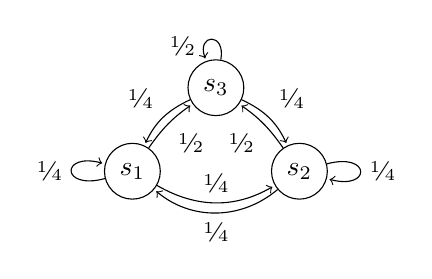
\begin{tikzpicture}[->,shorten >=1pt, node distance={15mm}, main/.style = {draw, circle}] 
    \node[main] (3) {$s_3$}; 
    \node[main] (1) [below left of=3] {$s_1$}; 
    \node[main] (2) [below right of=3]{$s_2$}; 

    \path
    (1) edge[bend left=-30] node[above] {\sfrac 1 4} (2)
        edge[bend right=-10] node[below right] {\sfrac 1 2} (3)
        edge[loop left] node[left] {\sfrac 1 4} (1);

    \path
    (2) edge[bend left=40] node[below] {\sfrac 1 4} (1)
        edge[bend left=-10] node[below left] {\sfrac 1 2} (3)
        edge[loop right] node[right] {\sfrac 1 4} (2);

    \path
    (3) edge[bend left=20] node[above right] {\sfrac 1 4} (2)
        edge[bend right=20] node[above left] {\sfrac 1 4} (1)
        edge[loop above,out=80,in=110,looseness=5] node[left=2mm,pos=0.2] {\sfrac 1 2} (3);

  \end{tikzpicture}
  \caption{Markov Process as a graph.}
  \label{fig:mdp_illustration}

\end{subfigure}
\begin{subfigure}[b]{0.69\textwidth}
  \centering
  \begin{align*}
    \pi = \begin{bmatrix}
      \sfrac 1 4 \\
      \sfrac 1 4 \\
      \sfrac 1 2 \\
    \end{bmatrix}, ~
    \Phi & = \begin{bmatrix}
      1 & 0 \\
      0 & -1 \\
      \sfrac{1}{2} (1.05 + \epsilon) & -\sfrac{1}{2} (1.05 + \epsilon)\\
    \end{bmatrix}, ~
    V = \begin{bmatrix}
      1 \\
      1 \\
      1.05 \\
    \end{bmatrix}
  \end{align*}
  \caption{Stationary distribution $\pi$, Value function basis $\Phi$, True state-values $V$}
  \label{fig:mdp_matrix}
\end{subfigure}

  \caption{Our three-state counter-example MDP. We use this to illustrate how the deadly triad problem persists despite common mitigating strategies. Rewards are set consistent with $V$, and the weights $\vec w$ are trained via TD to minimize $\|\Phi \vec w - V \|$. A small non-zero $\epsilon$ ensures there is some representation error to force the model to approximate the value function: $\|\Phi(\Phi^\top \Phi)^{-1}\Phi^\top V - V \| \leq \epsilon$. }
  \label{fig:mdp}
\end{figure}

\begin{figure}[!p]
    \begin{tikzpicture}
    \begin{axis}[
        scale only axis,
        width=\textwidth-10mm,
        height=5cm,
        tick align=outside,
        enlargelimits=false,
        ymode=log,
        mark=none,
        ymax=10,
        xlabel={$p$ in sampling distribution $\mu=[\sfrac p2, \sfrac p2, 1-p]$},
        yticklabels={,,},
        ylabel={TD error},
    ]
    \addplot[color=red,thick] table [x=p, y=err] {fixedpoint/eta_-infty.dat} node[below,pos=0.002] {$\eta=0$};
    \addplot[color=blue] table [x=p, y=err] {fixedpoint/eta_-6.dat} node[above,pos=0.01] {$\eta=10^{-6}$};
    \addplot[color=blue] table [x=p, y=err] {fixedpoint/eta_-4.dat} node[above,pos=0.022] {$\eta=10^{-4}$};
    \addplot[color=blue] table [x=p, y=err] {fixedpoint/eta_-2.dat} node[below,pos=0.1] {$\eta=10^{-2}$};
    \addplot[color=black,thick,dashed] table [x=p, y=err] {fixedpoint/eta_infty.dat} node[above,pos=0.06] {$\eta\to\infty$};
    %\legend{$\eta=0$,$\eta=10^{-6}$,$\eta=10^{-4}$,$\eta=10^{-2}$,$\eta=1$}
    \end{axis}
\end{tikzpicture}

    \caption{We plot TD error against $p$ for the MDP in Figure~\ref{fig:fixedpoint} with $\epsilon=10^{-4}$. This shape is characteristic of TD models in the presence of the deadly triad, including a minima close to $\pi$ ($p=0.5$), and an asymptote at the singular point ($p\approx 0.715$). At different levels of regularization the error function moves between the unregularized case ($\eta=0$) and the limiting case ($\eta\to\infty$).}
    \label{fig:fixedpoint}
\end{figure}


\begin{figure}
    \centering
\begin{subfigure}[b]{0.47\textwidth}
  \centering
  \label{fig:emp_weight}

  \begin{tikzpicture}
    \begin{axis}[
        scale only axis,
        width=\textwidth-10mm,
        height=4cm,
        tick align=outside,
        enlargelimits=false,
        mark=none,
        ymax=1.5,
        xlabel={distrib. param. $p$},
        ylabel={distrib. err. $\|\upsilon(\eta) - \pi\|$},
        yticklabels={,,},
        ylabel style={yshift = -9pt,},
    ]
    \addplot[color=red,very thick] table [x=p, y=err] {emphasistd/file_2a0.dat} node[below right,pos=0.7] {$\eta=0$};
    \addplot[color=black,dashed] table [x=p, y=err] {emphasistd/file_2a100..dat} node[above,pos=0.85] {$\eta\to\infty$};
    \addplot[color=blue,very thick] table [x=p, y=err] {emphasistd/file_2a0.0002.dat} node[below,pos=0.2] {$\eta=2\cdot 10^{-2}$};
    % Annotation:
    \addplot[color=red,only marks,mark=o,mark size=6pt] coordinates {(0.4,0)};
    \addplot[color=blue,only marks,mark=o,mark size=6pt] coordinates {(0.4,0.6123)};
    \draw[->,black,very thick,shorten >=6pt,shorten <=6pt] (0.4, 0) to [bend right] (0.4, 0.6123);
    \end{axis}
  \end{tikzpicture}
  \caption{distribution is $[\sfrac p2,~\sfrac p2,~(1-p)]$ }
  \label{fig:emphimp}
\end{subfigure}
\begin{subfigure}[b]{0.47\textwidth}
  \centering

  \begin{tikzpicture}
    \begin{axis}[
        scale only axis,
        width=\textwidth-10mm,
        height=4cm,
        tick align=outside,
        enlargelimits=false,
        mark=none,
        ymax=0.005,
        xlabel={distrib. param. $q$},
        ylabel={value err. $\|\Phi_v w_v^* - V\|$},
        yticklabels={,,},
        ylabel style={yshift = -9pt,},
    ]
    \addplot[color=black] table [x=p, y=err] {emphasistd/file_2b0.dat} node[below right,pos=0.7] {$\eta=0$};
    \draw[red,very thick] (0.5, 0.00086458) -- (0.5, 0.00086458|-{rel axis cs:0,0});
    \draw[red,dashed,very thick] (0.5, 0.005) -- (0.5, 0.005|-{rel axis cs:0,0});
    \draw[blue,very thick] (0.12, 0.005) -- (0.12, 0.005|-{rel axis cs:0,0});

    % Annotation:
    \addplot[color=red,only marks,mark=o,mark size=6pt] coordinates {(0.5,0.00086458)};
    \addplot[color=blue,only marks,mark=o,mark size=6pt] coordinates {(0.12,0.005)};
    \draw[->,black,very thick,shorten >=12pt,shorten <=6pt] (0.5, 0.00086458) to [] (0.12, 0.005);
    \end{axis}
  \end{tikzpicture}
  \caption{distribution is $[\sfrac {(1-q)}2,~\sfrac q2,~0.5]$ }
  \label{fig:emphval}
\end{subfigure}

    \caption{Ridge regularization distorts the emphasis model (left), which induces the value function (right) to move to a singularity. Ridge regularization can interact with emphasis models to significantly worsen learned value functions. (This example is with reference to the algorithm in \citep{zhang2021breaking}.) }
    \label{fig:emphasisplots}
\end{figure}

\clearpage

\appendix
\section*{Appendix }

\paragraph{Deadly-Triad instability}

The background to the instability is explained by \citet[p.~264]{sutton2020reinforcement}, and the linear case is analyzed in detail by \citet{kolter2011fixed}. The intuition behind this is that the TD fixed point when sampling on-policy is at the solution of the Bellman equation:
\begin{align}
\Phi \vec w & = R + \gamma\,P\,\Phi \vec w
\intertext{for feature basis $\Phi$, learned weights $\vec w$, reward function $R$, discount factor $\gamma$ and transition matrix $P$. However, when TD updates follow an off-policy distribution $\mu\in \mathbb R^n_0$, the TD solution is instead at the fixed point of the Bellman operator followed by a projection:}
\Phi \vec w & = \Pi_\mu \left( R + \gamma P \Phi \vec w \right)
\intertext{where $\Pi_\mu = \Phi (\Phi^\top D \Phi)^{-1} \Phi^\top D$ projects the Bellman backup onto the columnspace of $\Phi$, reweighted by the diagonal matrix $D = \text{diag}(\mu)$. This yields the closed-form solution:}
\vec w & = A^{-1} \vec b
\intertext{Where $A = \Phi^\top D (I - \gamma P) \Phi$ and $\vec b = \Phi^\top D R$. Under ridge regularization, some small $\eta$ is added to the diagonal of $A$ to ensure that the matrix being inverted is positive definite: }
\vec w & = (A + \eta I)^{-1} \vec b
\end{align}
The intuition behind the training instability is that, for some $\mu$, the matrix $A$ is ill-conditioned or singular, causing the inverse to become arbitrarily large or undefined.
This training instability occurs even when the bases $\Phi$ can almost exactly represent the value function, as illustrated in Figure~\ref{fig:fixedpoint}.

\paragraph{Adjacent Research Questions}
We may also pivot to answer some of these questions:

\begin{enumerate}
    \item With multi-layer networks, we can construct some examples in which some off-policy distributions are better than the on-policy distribution. What are the conditions for this and can we design an RL algorithm to exploit this?
    \item How common is deadly-triad caused instability in large RL problems? Which part of the problem structure is most likely to cause this, and can we transform the MDP to eliminate this possibility?
\end{enumerate}


\clearpage

% \bibliographystyle{plain}
\bibliography{biblio.bib}

\end{document}
 